% SPDX-License-Identifier: CC-BY-4.0
% feasibility-report.tex: 可行性报告

% Authors: 吴骏东 <1904346407@qq.com>,
%          张子辰 <zichen350@gmail.com>,
%          蓝俊玮 <ljw13@mail.ustc.edu.cn>,
%          郭耸霄 <logname@mail.ustc.edu.cn> and
%          陈建绿 <2512674094@qq.com>

% Copyright (C) 2022 吴骏东, 张子辰, 蓝俊玮, 郭耸霄 and 陈建绿
% All rights reserved.

% 🅭 🅯
% This document is licensed under a Creative Commons Attribution
% 4.0 International license <https://creativecommons.org/licenses/by/4.0/>.
\documentclass{../runikraft-report}

\hypersetup
{
  pdftitle={2022春 操作系统原理与设计(H) x-runikraft小组 可行性报告},
  pdfauthor={吴骏东; 张子辰; 蓝俊玮; 郭耸霄; 陈建绿}
}
\renewcommand{\today}{2022年4月23日}

\begin{document}
\title{\bfseries Runikraft小组\quad 可行性报告}
\author{吴骏东\and 张子辰\and 蓝俊玮\and 郭耸霄\and 陈建绿}
\date{\today}
\maketitle

\tableofcontents
\section{项目介绍}\sectionauthor{郭耸霄}
我们选择的课题是使用Rust语言改写Unikraft Unikernel。与RustyHermit和rCore等用Rust实现的操作系统不同,
我们将完全使用Rust的稳定特性编写代码。

众所周知,在互联网技术和云计算不断发展的今天,我们身边的虚拟化设备不断增多,
它们中的很多都使用了Unikernel。然而,虚拟化设备和Unikernel也暴露出了很多安全问题。
对这些安全问题,C语言因其本身的缺陷难辞其咎。

Rust 是一门让人人都能写出可靠、高效的软件的语言。\cite{7}利用Rust编写Unikernel,
可以充分发挥它相对C语言的高层抽象和内存安全保证。用Rust改写项目已经成为一种解决问题的
有效手段,如zalando公司从Scala转向Rust的成功故事。\cite{3}

RISC-V是一款自由、开源的ISA,它开启了全新的基于开放标准协作的处理器创新时代。\cite{0}
目前基于RISC-V架构的开源处理器有很多,既有标量处理器Rocket,
也有超标量处理器BOOM,还有面向嵌入式领域的Z-scale、PicoRV32等。\cite{2}

因此,我们计划使用Rust语言改写架构和性能方面占优的unikernel——Unikraft。
在这份报告中,我们将首先介绍项目的理论依据——Rust语言适用于系统编程的特性
及对Unikraft源码的分析和改写思路;随后,我们将介绍使用QEMU进行硬件仿真和
测试的方法;最后,我们将给出项目的创新点和总体设计。
\section{理论依据}
\subsection{Rust语言}\sectionauthor{陈建绿}\vspace*{-4ex}
\subsubsection{保证内存安全的方式}
在高级语言中,某个内存位置要在程序中能被访问,必然就会与一个或多个变量建立关联关系。
这会引出内存的不正确访问引发的内存安全问题。这些问题在C/C++中都是需要开发者非常小心地
自己处理。而 Rust 的语言特性则为上面的问题提供了解决方案。\cite{8}
\begin{table}[H]
\centering
\caption{Rust对内存安全问题的解决方案}
\begin{tabular}{|c|c|}
\hline
\textbf{问题} & \textbf{Rust 的解决方案}\\\hline
使用未初始化内存&编译器禁止读取未赋值变量\\\hline
对空指针解引用&使用\texttt{Option}枚举替代空指针\\\hline
悬垂指针&生命周期标识与编译器检查\\\hline
缓冲区溢出&编译器检查,拒绝超越缓冲区边界的数据访问\\\hline
非法释放内存&语言级的 RAII 机制,唯一的所有者才有权释放内存\\\hline
\end{tabular}
\end{table}
\subsubsection{保证线程安全的方式}
Rust 通过一整套设计非常精良的基础设施来保证这一点,这些基础设施配合类型检查和
借用模型“强迫”程序员写出正确的代码,把别的语言在运行时的崩溃或泄露暴露在编译期,
从而保证线程安全。

\noindent 基础设施:

\begin{enumerate}
\item 进行语义限制的\texttt{Send} / \texttt{Sync} 、\texttt{Trait}。
\item 共享不可变所有权的\texttt{Arc} (\texttt{Rc}的多线程版本)。
\item 提供内部可变性的\texttt{Mutex} / \texttt{Rwlock}。
\item 管道模型\texttt{channel}。
\item 其他的一些线程相关的API。
\end{enumerate}

\noindent 线程相关的常见API与设施:

\begin{enumerate}
\item \texttt{std::thread::spawn},\texttt{spawn}接收一个闭包并执行,返回一个
\texttt{JoinHandle}类型的值,它拥有线程所有权;
\item  \texttt{join()}函数,该函数作用在线程句柄\texttt{JoinHandle}类型的值上,
使得父线程能够等待子线程执行完毕;
\item \texttt{move}+闭包,\texttt{move}闭包常常与\texttt{thread}和\texttt{spawn}
一起使用,它允许我们在一个线程中使用另外一个线程的数据,使用\texttt{move}关键字强制闭包获取
其使用的环境值的所有权。
\end{enumerate}

Rust 所拥有的这些设施以及自身的特性可以让我们编写出正确的代码从而保证线程安全。\cite{9}

\subsubsection{Unsafe Rust}
在进行底层系统编程时,我们必须要使用Rust 的unsafe关键字,使用该关键字可以使我们实现以下功能:

解引用原生指针,这对于和C语言和汇编语言程序交互很有用。
调用一个不安全的函数或方法(例如C语言函数)。
访问和修改静态变量,后者是Rust中的"全局变量"。
使用Unsafe Rust会在一定程度上减少Rust编译器的安全检查,但牺牲的稍许安全性却可以换来
灵活性的巨大提高。在与硬件抽象进行交互时,我们可能
需要使用这个特性。

\subsection{Rust与C交互}
Rust 中提供了\texttt{extern}关键字来简化创建和使用外部接口(Foreign Function
Interface, FFI)的过程。FFI 是编程语言定义函数的一种方式,它允许其他(外部的)编程语言
来调用这些函数。
下面是一个集成了C标准库中的\texttt{abs}函数的示例代码:
\begin{lstlisting}[numbers=left]
	extern "C" {
		fn abs(input: i32) -> i32;
	}
	fn main(){
		unsafe {
			println!("Absolue value of -3 according to C: {}", abs(-3));
		}
	}
\end{lstlisting}
这段代码在\texttt{extern "C"}块中列出了它想要调用的外部函数和签名,其中的\texttt{"C"}指明
了外部函数使用的应用二进制接口(Application Binary Interface, ABI):它被用来定义函数在
汇编层面的调用方式。

要在其他语言中调用 Rust 函数,同样可以使用\texttt{extern}来创建一个允许其他语言调用 Rust
函数的接口。创建时需要将\texttt{extern}关键字及对应的 ABI 添加到函数签名的\texttt{fn}关键字
前,并为该函数添加\texttt{\#[no\_mangle]}注解来避免 Rust 在编译时改变它的名称。
下面是一个可以在编译并链接后被 C 语言代码访问的函数定义:
\begin{lstlisting}[numbers=left,language=Rust]
	#[no_mangle]
	pub extern "C" fn call_from_c() {
		println!("Just called a Rust function from C!");
	}
\end{lstlisting}
这一类型的\texttt{extern}功能不需要使用\texttt{unsafe}。

\subsection{Rust的条件编译}\label{subsec:cond-compile}
Rust通过cfg属性,对条件编译提供了支持。这些配置在Cargo.toml中提供,例如:

\begin{lstlisting}[numbers=left,language=Rust]
[features]
# no features by default
default = []

# The “secure-password” feature depends on the bcrypt package.
secure-password = ["bcrypt"]

# A feature with no dependencies is used mainly for conditional compilation, like `#[cfg(feature = "go-faster")]`.
go-faster = []
\end{lstlisting}

在代码中,可以采用cfg属性修饰函数:
\begin{lstlisting}[numbers=left,language=Rust]
// This function is only included when compiling for a unixish OS with a 32-bit architecture
#[cfg(all(unix, target_pointer_width = "32"))]
fn on_32bit_unix() {
	// ...
}
\end{lstlisting}
也可以使用以下类似\texttt{\#\textbf{ifdef}}的方式进行条件编译:
\begin{lstlisting}[numbers=left,language=Rust]
let machine_kind = if cfg!(unix) {
	"unix"
} else if cfg!(windows) {
	"windows"
} else {
	"unknown"
};

println!("I'm running on a {} machine!", machine_kind);
\end{lstlisting}
\cite{e}

\subsection{RISC-V ISA}\sectionauthor{吴骏东}\vspace*{-4ex}
\subsubsection{特权特权模型}
在编写unikernel时,我们需要使用特权指令处理外设中断、控制机器状态,
因此需要了解RISC-V的特权模型。

截至目前(2022.4),RISC-V 共定义了四个特权级别,由高到低排列顺次为:

\begin{description}
\item[机器级别(M)] RISC-V中硬件线程可以执行的最高权限模式。
在M模式下运行的 hart 对内存、I/O 和一些对于启动和配置系统来说必要的底层
功能有着完全的使用权。因此它是唯一所有标准 RISC-V 处理器都必须实现的权限模式。\cite{a}
\item[超级监管者级别(H)] 为了支持虚拟机监视器。但目前该级别并没有被正式加入到文档中。
\item[监管者级别(S)] 为了支持现代操作系统,如 Linux,FreeBSD 和 Windows 。
\item[用户级别(U)] 用于运行应用程序,适用于安全嵌入式系统。
\end{description}

标准的 RISC-V 为超过4000个 CSR 预留了12位的编码空间(\texttt{[11:0]})。
其中,\texttt{[11:8]} 位根据特权级别对 CSR 的读写权限进行编码。
注意:任何试图访问不存在的 CSR 的行为均会引发指令异常,尝试写入只读寄存器也会引发指令异常。
剩余的8位编码 \texttt{[7:0]} 将指定相应的寄存器地址位置。具体细节如下所示:\cite{b}\cite{c}

\begin{lstlisting}[numbers=left]
CSR [11:10]:对读写模式进行约束
00		read/write
01		read/write
10		read/write
11		read-only
CSR [9:8]:对访问最低权限进行约束
00		Unprivileged and User-Level CSRs
01		Supervisor-Level CSRs
10		Hypervisor and VS CSRs
11		Machine-Level CSRs
\end{lstlisting}


目前 RISC-V 支持的特权指令格式为:
%\begin{table}[H]
    %\caption{RISC-V 特权指令}
{
    \small
    \newcommand{\instbit}[1]{\mbox{\scriptsize #1}}
    \newcommand{\instbitrange}[2]{~\instbit{#1} \hfill \instbit{#2}~}
    %\centering

    \begin{longtable}{p{0in}p{0.4in}p{0.05in}p{0.05in}p{0.05in}p{0.05in}p{0.4in}p{0.6in}p{0.4in}p{0.6in}p{0.7in}l}
    \caption{RISC-V 特权指令}\\
    &
    \multicolumn{1}{l}{\instbit{31}} &
    \multicolumn{1}{r}{\instbit{27}} &
    \instbit{26} &
    \instbit{25} &
    \multicolumn{1}{l}{\instbit{24}} &
    \multicolumn{1}{r}{\instbit{20}} &
    \instbitrange{19}{15} &
    \instbitrange{14}{12} &
    \instbitrange{11}{7} &
    \instbitrange{6}{0} \\
    \cline{2-11}
    \endfirsthead
    &
    \multicolumn{1}{l}{\instbit{31}} &
    \multicolumn{1}{r}{\instbit{27}} &
    \instbit{26} &
    \instbit{25} &
    \multicolumn{1}{l}{\instbit{24}} &
    \multicolumn{1}{r}{\instbit{20}} &
    \instbitrange{19}{15} &
    \instbitrange{14}{12} &
    \instbitrange{11}{7} &
    \instbitrange{6}{0} \\
    \cline{2-11}
    \endhead

    &
    \multicolumn{4}{|c|}{funct7} &
    \multicolumn{2}{c|}{rs2} &
    \multicolumn{1}{c|}{rs1} &
    \multicolumn{1}{c|}{funct3} &
    \multicolumn{1}{c|}{rd} &
    \multicolumn{1}{c|}{opcode} & R-type \\
    \cline{2-11}


    &
    \multicolumn{6}{|c|}{imm[11:0]} &
    \multicolumn{1}{c|}{rs1} &
    \multicolumn{1}{c|}{funct3} &
    \multicolumn{1}{c|}{rd} &
    \multicolumn{1}{c|}{opcode} & I-type \\
    \cline{2-11}


    &
    \multicolumn{10}{c}{} & \\
    &
    \multicolumn{10}{c}{\bf Trap-Return Instructions} & \\
    \cline{2-11}


    &
    \multicolumn{4}{|c|}{0001000} &
    \multicolumn{2}{c|}{00010} &
    \multicolumn{1}{c|}{00000} &
    \multicolumn{1}{c|}{000} &
    \multicolumn{1}{c|}{00000} &
    \multicolumn{1}{c|}{1110011} & SRET \\
    \cline{2-11}


    &
    \multicolumn{4}{|c|}{0011000} &
    \multicolumn{2}{c|}{00010} &
    \multicolumn{1}{c|}{00000} &
    \multicolumn{1}{c|}{000} &
    \multicolumn{1}{c|}{00000} &
    \multicolumn{1}{c|}{1110011} & MRET \\
    \cline{2-11}


    &
    \multicolumn{10}{c}{} & \\
    &
    \multicolumn{10}{c}{\bf Interrupt-Management Instructions} & \\
    \cline{2-11}


    &
    \multicolumn{4}{|c|}{0001000} &
    \multicolumn{2}{c|}{00101} &
    \multicolumn{1}{c|}{00000} &
    \multicolumn{1}{c|}{000} &
    \multicolumn{1}{c|}{00000} &
    \multicolumn{1}{c|}{1110011} & WFI \\
    \cline{2-11}


    &
    \multicolumn{10}{c}{} & \\
    &
    \multicolumn{10}{c}{\bf Supervisor Memory-Management Instructions} & \\
    \cline{2-11}


    &
    \multicolumn{4}{|c|}{0001001} &
    \multicolumn{2}{c|}{rs2} &
    \multicolumn{1}{c|}{rs1} &
    \multicolumn{1}{c|}{000} &
    \multicolumn{1}{c|}{00000} &
    \multicolumn{1}{c|}{1110011} & SFENCE.VMA \\
    \cline{2-11}


    &
    \multicolumn{10}{c}{} & \\
    &
    \multicolumn{10}{c}{\bf Hypervisor Memory-Management Instructions} & \\
    \cline{2-11}


    &
    \multicolumn{4}{|c|}{0010001} &
    \multicolumn{2}{c|}{rs2} &
    \multicolumn{1}{c|}{rs1} &
    \multicolumn{1}{c|}{000} &
    \multicolumn{1}{c|}{00000} &
    \multicolumn{1}{c|}{1110011} & HFENCE.VVMA \\
    \cline{2-11}


    &
    \multicolumn{4}{|c|}{0110001} &
    \multicolumn{2}{c|}{rs2} &
    \multicolumn{1}{c|}{rs1} &
    \multicolumn{1}{c|}{000} &
    \multicolumn{1}{c|}{00000} &
    \multicolumn{1}{c|}{1110011} & HFENCE.GVMA \\
    \cline{2-11}


    &
    \multicolumn{10}{c}{} & \\
    &
    \multicolumn{10}{c}{\bf Hypervisor Virtual-Machine Load and Store Instructions} & \\
    \cline{2-11}


    &
    \multicolumn{4}{|c|}{0110000} &
    \multicolumn{2}{c|}{00000} &
    \multicolumn{1}{c|}{rs1} &
    \multicolumn{1}{c|}{100} &
    \multicolumn{1}{c|}{rd} &
    \multicolumn{1}{c|}{1110011} & HLV.B \\
    \cline{2-11}


    &
    \multicolumn{4}{|c|}{0110000} &
    \multicolumn{2}{c|}{00001} &
    \multicolumn{1}{c|}{rs1} &
    \multicolumn{1}{c|}{100} &
    \multicolumn{1}{c|}{rd} &
    \multicolumn{1}{c|}{1110011} & HLV.BU \\
    \cline{2-11}


    &
    \multicolumn{4}{|c|}{0110010} &
    \multicolumn{2}{c|}{00000} &
    \multicolumn{1}{c|}{rs1} &
    \multicolumn{1}{c|}{100} &
    \multicolumn{1}{c|}{rd} &
    \multicolumn{1}{c|}{1110011} & HLV.H \\
    \cline{2-11}


    &
    \multicolumn{4}{|c|}{0110010} &
    \multicolumn{2}{c|}{00001} &
    \multicolumn{1}{c|}{rs1} &
    \multicolumn{1}{c|}{100} &
    \multicolumn{1}{c|}{rd} &
    \multicolumn{1}{c|}{1110011} & HLV.HU \\
    \cline{2-11}


    &
    \multicolumn{4}{|c|}{0110100} &
    \multicolumn{2}{c|}{00000} &
    \multicolumn{1}{c|}{rs1} &
    \multicolumn{1}{c|}{100} &
    \multicolumn{1}{c|}{rd} &
    \multicolumn{1}{c|}{1110011} & HLV.W \\
    \cline{2-11}


    &
    \multicolumn{4}{|c|}{0110010} &
    \multicolumn{2}{c|}{00011} &
    \multicolumn{1}{c|}{rs1} &
    \multicolumn{1}{c|}{100} &
    \multicolumn{1}{c|}{rd} &
    \multicolumn{1}{c|}{1110011} & HLVX.HU \\
    \cline{2-11}


    &
    \multicolumn{4}{|c|}{0110100} &
    \multicolumn{2}{c|}{00011} &
    \multicolumn{1}{c|}{rs1} &
    \multicolumn{1}{c|}{100} &
    \multicolumn{1}{c|}{rd} &
    \multicolumn{1}{c|}{1110011} & HLVX.WU \\
    \cline{2-11}


    &
    \multicolumn{4}{|c|}{0110001} &
    \multicolumn{2}{c|}{rs2} &
    \multicolumn{1}{c|}{rs1} &
    \multicolumn{1}{c|}{100} &
    \multicolumn{1}{c|}{00000} &
    \multicolumn{1}{c|}{1110011} & HSV.B \\
    \cline{2-11}


    &
    \multicolumn{4}{|c|}{0110011} &
    \multicolumn{2}{c|}{rs2} &
    \multicolumn{1}{c|}{rs1} &
    \multicolumn{1}{c|}{100} &
    \multicolumn{1}{c|}{00000} &
    \multicolumn{1}{c|}{1110011} & HSV.H \\
    \cline{2-11}


    &
    \multicolumn{4}{|c|}{0110101} &
    \multicolumn{2}{c|}{rs2} &
    \multicolumn{1}{c|}{rs1} &
    \multicolumn{1}{c|}{100} &
    \multicolumn{1}{c|}{00000} &
    \multicolumn{1}{c|}{1110011} & HSV.W \\
    \cline{2-11}


    &
    \multicolumn{10}{c}{} & \\
    &
    \multicolumn{10}{c}{\bf Hypervisor Virtual-Machine Load and Store Instructions, RV64 only} & \\
    \cline{2-11}


    &
    \multicolumn{4}{|c|}{0110100} &
    \multicolumn{2}{c|}{00001} &
    \multicolumn{1}{c|}{rs1} &
    \multicolumn{1}{c|}{100} &
    \multicolumn{1}{c|}{rd} &
    \multicolumn{1}{c|}{1110011} & HLV.WU \\
    \cline{2-11}


    &
    \multicolumn{4}{|c|}{0110110} &
    \multicolumn{2}{c|}{00000} &
    \multicolumn{1}{c|}{rs1} &
    \multicolumn{1}{c|}{100} &
    \multicolumn{1}{c|}{rd} &
    \multicolumn{1}{c|}{1110011} & HLV.D \\
    \cline{2-11}


    &
    \multicolumn{4}{|c|}{0110111} &
    \multicolumn{2}{c|}{rs2} &
    \multicolumn{1}{c|}{rs1} &
    \multicolumn{1}{c|}{100} &
    \multicolumn{1}{c|}{00000} &
    \multicolumn{1}{c|}{1110011} & HSV.D \\
    \cline{2-11}


    &
    \multicolumn{10}{c}{} & \\
    &
    \multicolumn{10}{c}{\bf \emph{Svinval} Memory-Management Extension} & \\
    \cline{2-11}


    &
    \multicolumn{4}{|c|}{0001011} &
    \multicolumn{2}{c|}{rs2} &
    \multicolumn{1}{c|}{rs1} &
    \multicolumn{1}{c|}{000} &
    \multicolumn{1}{c|}{00000} &
    \multicolumn{1}{c|}{1110011} & SINVAL.VMA \\
    \cline{2-11}


    &
    \multicolumn{4}{|c|}{0001100} &
    \multicolumn{2}{c|}{00000} &
    \multicolumn{1}{c|}{00000} &
    \multicolumn{1}{c|}{000} &
    \multicolumn{1}{c|}{00000} &
    \multicolumn{1}{c|}{1110011} & SFENCE.W.INVAL \\
    \cline{2-11}


    &
    \multicolumn{4}{|c|}{0001100} &
    \multicolumn{2}{c|}{00001} &
    \multicolumn{1}{c|}{00000} &
    \multicolumn{1}{c|}{000} &
    \multicolumn{1}{c|}{00000} &
    \multicolumn{1}{c|}{1110011} & SFENCE.INVAL.IR \\
    \cline{2-11}


    &
    \multicolumn{4}{|c|}{0010011} &
    \multicolumn{2}{c|}{rs2} &
    \multicolumn{1}{c|}{rs1} &
    \multicolumn{1}{c|}{000} &
    \multicolumn{1}{c|}{00000} &
    \multicolumn{1}{c|}{1110011} & HINVAL.VVMA \\
    \cline{2-11}


    &
    \multicolumn{4}{|c|}{0110011} &
    \multicolumn{2}{c|}{rs2} &
    \multicolumn{1}{c|}{rs1} &
    \multicolumn{1}{c|}{000} &
    \multicolumn{1}{c|}{00000} &
    \multicolumn{1}{c|}{1110011} & HINVAL.GVMA \\
    \cline{2-11}


    \end{longtable}
}

以 CSR 访存指令为例。其标准格式为:
\begin{table}[H]
    \centering
    \caption{状态控制寄存器(CSR)}
    \begin{tabular}{|r|c|>{\ttfamily}l>{\ttfamily}l|}
        \hline
        读/写&I&CSRRW&rd,csr,rs1\\
        读\&设置位&I&CSRRS&rd,csr,rs1\\
        读\&清除位&I&CSRRC&rd,csr,rs1\\
        读/写\ 立即数&I&CSRRWI&rd,csr,imm\\
        读\&设置位\ 立即数&I&CSRRSI&rd,csr,imm\\
        读\&清除位\ 立即数&I&CSRRCI&rd,csr,imm\\\hline
    \end{tabular}
\end{table}

除目前 RISC-V 支持的特权指令格式外,\texttt{ecall}指令用于系统调用。

\subsubsection{监管者二进制接口}
为了降低S模式的程序在不同RISC-V的设备之间的移植难度,
RISC-V引入了监管者二进制接口(\textbf{S}upervisor \textbf{B}inary \textbf{I}nterface)。
它在M模式运行,为运行在S模式下的操作系统内核提供硬件抽象。

与U模式的程序使用系统调用陷入S模式类似,S模式的系统内核也可以用SBI调用陷入M模式,
以使用SBI提供的服务。

\begin{figure}[tbh!]
\centering
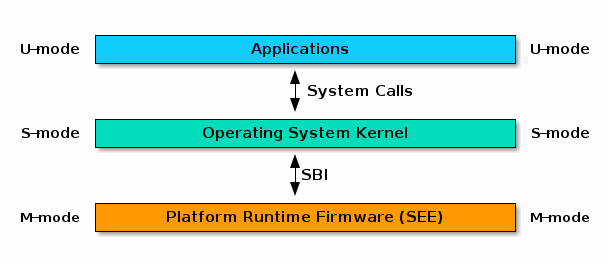
\includegraphics[width=0.7\linewidth]{assets/riscv-sbi-intro1.png}
\caption{不含H拓展的RISC-V系统}
\label{fig:riscv-sbi}
\end{figure}

如下为\texttt{arch/riscv/kernel/sbi.c}中的部分代码,使用\texttt{ecall}指令时,
将EID写在\texttt{a7} 寄存器,FID写在\texttt{a6}寄存器,参数写在 \texttt{a0}-\texttt{a5} 寄存器,
后面会根据EID和FID的不同调用不同的处理函数。
\begin{lstlisting}[language=C,numbers=left]
struct sbiret sbi_ecall(int ext, int fid, unsigned long arg0,
unsigned long arg1, unsigned long arg2,
unsigned long arg3, unsigned long arg4,
unsigned long arg5)
{
	struct sbiret ret;

	register uintptr_t a0 asm ("a0") = (uintptr_t)(arg0);
	register uintptr_t a1 asm ("a1") = (uintptr_t)(arg1);
	register uintptr_t a2 asm ("a2") = (uintptr_t)(arg2);
	register uintptr_t a3 asm ("a3") = (uintptr_t)(arg3);
	register uintptr_t a4 asm ("a4") = (uintptr_t)(arg4);
	register uintptr_t a5 asm ("a5") = (uintptr_t)(arg5);
	register uintptr_t a6 asm ("a6") = (uintptr_t)(fid);
	register uintptr_t a7 asm ("a7") = (uintptr_t)(ext);
	asm volatile ("ecall"
	: "+r" (a0), "+r" (a1)
	: "r" (a2), "r" (a3), "r" (a4), "r" (a5), "r" (a6), "r" (a7)
	: "memory");
	ret.error = a0;
	ret.value = a1;

	return ret;
}
\end{lstlisting}​

例如可以用如下程序实现一个打印一个字符到系统控制台上的\texttt{putchar}函数:
\begin{lstlisting}[language=C]
    void sbi_console_putchar(int ch)
    {
    	sbi_ecall(SBI_EXT_0_1_CONSOLE_PUTCHAR, 0, ch, 0, 0, 0, 0, 0);
    }
\end{lstlisting}

用SBI可以降低开发系统的难度,但是会引入\texttt{ecall}指令,而unikernel的高效正是
依靠避免\texttt{ecall}实现的,所以我们只会在前期使用SBI提供的服务,后期会用自己编写
的virtio驱动程序代替SBI。


\subsubsection{KVM对RISC-V架构的支持}
KVM (Kernel-based Virtual Machine,基于内核的虚拟机)  ,是一种内建于 Linux 中的
开源虚拟化技术。具体而言,KVM 可以将 Linux 转变为虚拟监控程序,从而使主机计算机能够运行
多个隔离的虚拟环境,即虚拟客户机或虚拟机(VM)。
\begin{figure}[!hbt]
	\centering
	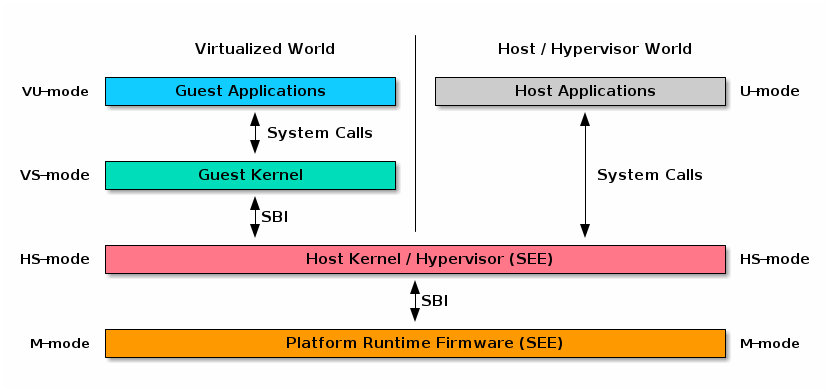
\includegraphics[width=0.9\linewidth]{assets/riscv-sbi-intro2.png}
	\caption{虚拟化下的特权等级}
	\label{fig:w4}
\end{figure}

如图\ref{fig:w4},为了支持虚拟化,RISC-V 规范定义了 RISC-V H-extension ,在原来的3级
特权架构的基础上对原有的 Supervisor 模式进行了扩展,引入了 Hypervisor-Extended Supervisor mode(HS)。
此时,在 Machine Mode 下运行最高优先级的、对全部资源具备操作能力的 Firmware ,虚拟机软件
Hypervisor 运行在 HS 模式,虚拟机 VM 运行在虚拟化的 Supervisor 模式,应用程序继续运行在
虚拟操作系统之上,运行在 Virtualized User mode。

为了实现 Supervisor 与 Hypervisor-extended supervisor 模式的切换,RSIC-V 将原来
Supervisor 模式下的 CSR 复制一份到Hypervisor,从而让每个硬件线程拥有两份 supervisor
寄存器,加快两个模式之间的切换过程。

由于 RISC-V 没有为不同虚拟化软件设计专门的特权模式,而是设计了统一的特权模式,这说明它对
1类(如Xvisor)、 2类(如KVM)虚拟化软件都有很好的支持。 RISC-V 可以通过 CSR 寄存器注入
中断,因此不需要为虚拟化而特殊设计中断控制器外设。此外,RISC-V 可直接借助特殊的寄存器位支持
嵌套虚拟化,而 Aarch64 要等到 v8.3 版本之后才支持这个功能。RISC-V 的时钟和核间中断可通过
SBI 软件辅助完成,而 Aarch64 需要特殊设计的计时器外设来支持虚拟化功能。\cite{d}

\subsection{QEMU}\sectionauthor{吴骏东}

QEMU是一款通用、开源的机器模拟器和虚拟化器。

当用作机器模拟器时,QEMU可以把一个机器(如ARM board)的系统或程序运行在不同的机器上(如你的PC)。
借助动态翻译,它达到了非常好的性能。

当用作虚拟化器时,QEMU通过直接在宿主机CPU上运行客户机代码,达到了接近原生的性能。QEMU支持两种模式
的虚拟化:在Xen hypervisor下执行,或者使用Linux内核模块KVM。当使用KVM时,QEMU可以虚拟化x86、
服务器和嵌入PowerPC、64位 POWER、S390、32位和64位ARM、RISC-V\cite{qemu7}以及MIPS客户机。\cite{1}

\noindent QEMU具有如下优点:

\begin{description}
\item[完整系统的模拟] Run operating systems for any machine, on any supported architecture.
\item[用户态的模拟] Run programs for another Linux/BSD target, on any supported architecture.
\item[虚拟化] Run KVM and Xen virtual machines with near native performance.\cite{1}
\end{description}

\subsection{Unikraft架构分析}\sectionauthor{张子辰}\vspace*{-4ex}
\subsubsection{代码风格}\label{ssubsec:code-style}
Unikraft的代码组织方式充分体现了模块化设计,核心代码被放在了\texttt{arch/}、\texttt{include/}和
\texttt{plat/}三个目录下,而系统的几乎所有功能都由位于\texttt{lib/}目录下的micro-libraries提供。
一个micro-library被放在一个目录下:
\begin{itemize}
\item \texttt{include/}:micro-library的API;
\item \texttt{Config.uk}:menu-config配置;
\item \texttt{exportsyms.uk}:导出的符号;
\item \texttt{Makefile.uk}:自动构建系统的配置;
\item \texttt{*.c}:micro-library的实现。
\item \texttt{extra.ld}:(可选)链接器配置。
\end{itemize}

比如,\texttt{uksched}的目录结构:
{\linespread{1}
\begin{verbatim}
    uksched
    ├── Config.uk
    ├── exportsyms.uk
    ├── extra.ld
    ├── include
    │   └── uk
    │       ├── sched.h
    │       ├── thread_attr.h
    │       ├── thread.h
    │       ├── wait.h
    │       └── wait_types.h
    ├── Makefile.uk
    ├── sched.c
    ├── thread_attr.c
    └── thread.c
\end{verbatim}}

Unikraft用UNIX命名风格,函数名和结构体
以\texttt{uk\_\hspace{0cm}\textit{<micro-library\hspace{0cm}名\hspace{0cm}>}\hspace{0cm}\_}
开头,结构体名后\textit{通常}附加\texttt{\_t},
比如\texttt{uk\_malloc}、\texttt{uk\_alloc\_malloc\_func\_t}。
Unikraft使用面向对象设计,每个micro-library中通常有与库同名的结构体,如\texttt{uk\_sched},
库中的函数的第一个参数通常是执行这个结构体的指针,如
\texttt{\textbf{struct} uk\_sched *uk\_sched\_create(\textbf{struct} uk\_alloc *a, \textbf{size\_t} prv\_size)}。

\subsubsection{编译运行流程}
以编译\href{https://github.com/unikraft/app-helloworld}{hello world程序}为例,介绍编译并
运行基于Unikraft的unikernel的流程。

首先要修改\texttt{Makefile},把\texttt{UK\_ROOT}改为unikraft源代码的目录,比如
\texttt{UK\_ROOT ?= \linebreak\$(PWD)/../unikraft},当然也可以不修改\texttt{Makefile}而修改
命令行参数。

用\texttt{make menuconfig}配置,然后用\texttt{make}编译。
\begin{figure}[!hbt]
\centering
\vspace*{-3ex}
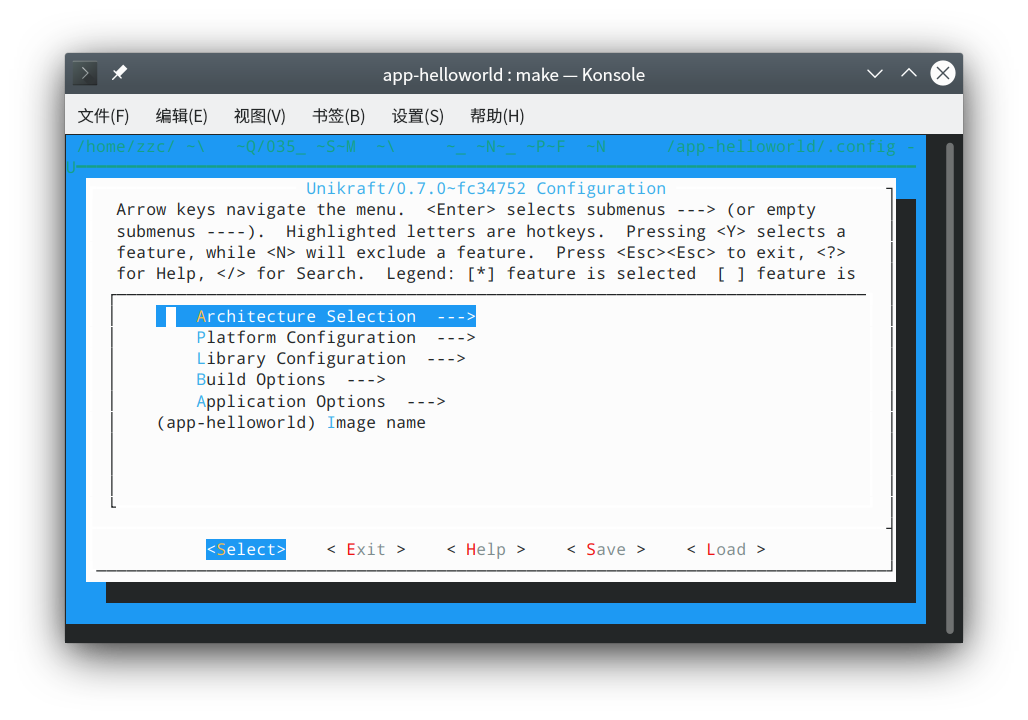
\includegraphics[width=0.9\linewidth]{assets/unikraft-menuconfig}
\vspace*{-3ex}
\caption{配置Unikraft}
\label{fig:unikraft-menuconfig}
\end{figure}
Hello world程序与Unikraft的各个被使用的micro-libraries先被分别编译成了\texttt{.o}文件,
再链接成一个unikernel镜像。一共生成了\texttt{libkvmplat}、\texttt{libkvmpci}、\texttt{libkvmvirtio}、
\texttt{apphelloworld}、\texttt{libnolibc}、\texttt{libukalloc}、\texttt{libukallocbbuddy}、
\texttt{libukargparse}、\texttt{libukboot}、\texttt{libukbus}、\texttt{libukdebug}、
\texttt{libuksglist}、\texttt{libuktime}、\texttt{libuktimeconv}和\texttt{libx86\_64arch}等中间文件。
最后的输出是18.0KiB大的\texttt{app-\linebreak helloworld\_kvm-x86\_64.gz}。

详细的编译日志位于我们的仓库的\href{https://github.com/OSH-2022/x-runikraft/tree/d22ccf0c1b248667148fd8953b71b6e0258de6a3/reference/Unikraft%20helloworld}{reference/Unikraft helloworld/}目录。

用\texttt{qemu-system-x86\_64 -kernel build/app-helloworld\_kvm-x86\_64 -nographic}\linebreak 运行hello world程序。

\begin{figure}[tbh!]
\centering
\vspace*{-3ex}
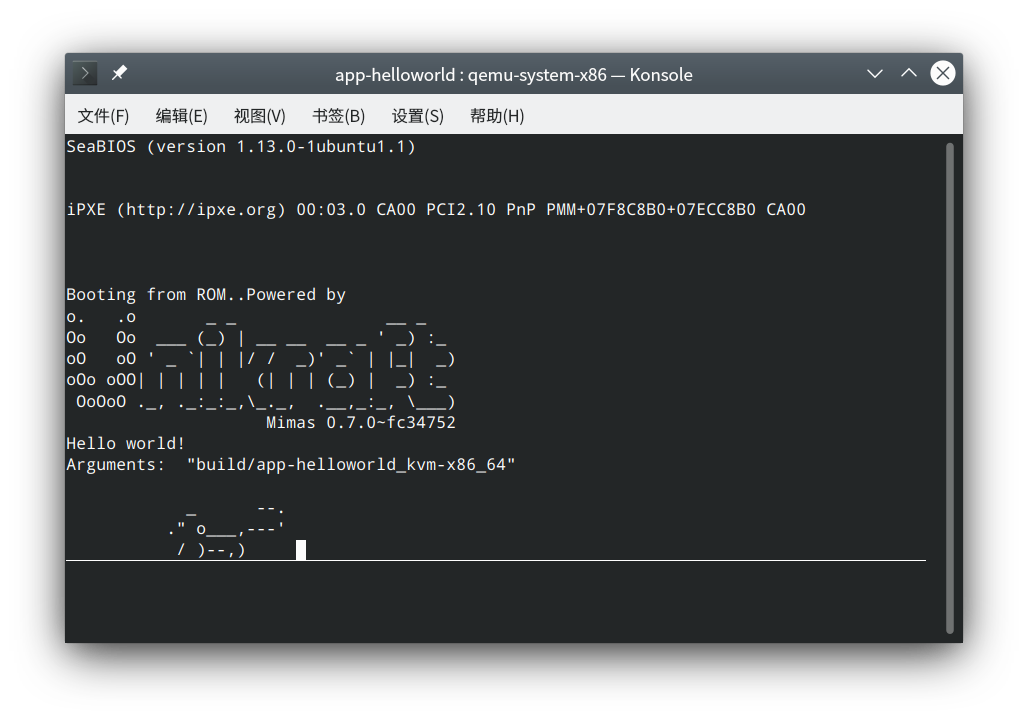
\includegraphics[width=0.9\linewidth]{assets/unikraft-run}
\vspace*{-3ex}
\caption{运行hello world}
\label{fig:unikraft-run}
\end{figure}


\subsubsection[开机流程]{开机流程(KVM+AMD64)}
\begin{enumerate}
\item bootloader(由虚拟机的固件实现)。
\item \texttt{\_libkvmplat\_start32}(位于\texttt{plat/kvm/x86/entry64.S}):
    \begin{enumerate}
    \item enable pae;
    \item enable long mode;
    \item load pml4 pointer;
    \item enable paging;
    \item \texttt{jmp \_libkvmplat\_start64}。
    \end{enumerate}
\item \texttt{\_libkvmplat\_start64}:
    \begin{enumerate}
    \item 一系列复杂的初始化;
    \item \texttt{call \_libkvmplat\_entry}。
    \end{enumerate}
\item \texttt{\_libkvmplat\_entry}(位于\texttt{plat/kvm/x86/setup.c}),
它接受\texttt{struct multiboot\_info*}参数:
    \begin{enumerate}
    \item \texttt{\_init\_cpufeatures};
    \item \texttt{\_libkvmplat\_init\_console};
    \item \texttt{traps\_init};
    \item \texttt{intctrl\_init};
    \item \texttt{\_mb\_get\_cmdline}:把multiboot\_info中的命令行参数复制到数据段
    的\texttt{char\linebreak cmdline[8192]};
    \item \texttt{\_mb\_init\_mem}:处理与内存分段有关的操作;
    \item \texttt{\_mb\_init\_initrd`};
    \item (\texttt{CONFIG\_HAVE\_SMP})\footnote{表示在开启某个配置时执行。} \texttt{acpi\_init};
    \item (\texttt{CONFIG\_HAVE\_SYSCALL}) \texttt{\_init\_syscall};
    \item (\texttt{CONFIG\_HAVE\_X86PKU}) \texttt{\_check\_ospke};
    调用\texttt{\_libkvmplat\_newstack}从引导栈切换走。
    \end{enumerate}
    可以看出,AMD64的开机流程很复杂,在ARMv8中,系统的起点是用汇编语言编写
    的\texttt{\_libkvmplat\_entry},它调用用C语言编写的\texttt{\_libkvmplat\_start},
    之后的流程与AMD64相同。
\item \texttt{\_libkvmplat\_entry2}:把cmdline传递给\texttt{ukplat\_entry\_argp}。
\item \texttt{ukplat\_entry\_argp}:把命令行参数拆成argc+argv的形式,然后调用\texttt{ukplat\_entry}。
\item \texttt{ukplat\_entry}:
    \begin{enumerate}
    \item 调用\texttt{ctorfn}注册的构造函数(\texttt{ctors.h}提供了注册构造函数的机制);
    \item (\texttt{CONFIG\_LIBUKLIBPARAM})进一步分析命令行参数;
    \item (\texttt{!CONFIG\_LIBUKBOOT\_NOALLOC}) 依次尝试在每一块内存区域上初始化
    分配器\linebreak(\texttt{uk\_<name>\_init}),
    成功创建分配器后,将剩余的内存区域加入分配器\linebreak(\texttt{uk\_alloc\_addmem});
    \item (\texttt{CONFIG\_LIBUKALLOC}) 初始化中断(\texttt{ukplat\_irq\_init});
    \item (\texttt{CONFIG\_LIBUKSCHED}) 初始化调度器\texttt{uk\_sched\_default\_init};
    \item (\texttt{CONFIG\_LIBUKSCHED}?)
        \begin{itemize}
        \item (true)  创建主线程(执行\texttt{main\_thread\_func})→启动调度器(\texttt{uk\_sched\_start}),
        \item (false) 启动中断(\texttt{ukplat\_lcpu\_enable\_irq})→直接调用\texttt{main\_thread\_func}。
        \end{itemize}
    \end{enumerate}
\item \texttt{main\_thread\_func}:
    \begin{enumerate}
    \item 调用init table上注册的函数(由\texttt{init.h}提供,与\texttt{ctorfn}类似);
    \item (\texttt{CONFIG\_LIBUKSP})\texttt{uk\_stack\_chk\_guard\_setup};
    \item 调用用户程序的构造函数 \texttt{\_\_preinit\_array}和\texttt{\_\_init\_array};
    \item 调用用户程序的\texttt{main}。
    \end{enumerate}
\item \texttt{main}。
\item 关机/崩溃。
\end{enumerate}

\subsubsection{分配器}
分配器的API位于\texttt{ukalloc},可选的实现有\texttt{ukallocbbuddy}、\texttt{ukallocpool}、
\texttt{ukallocregion}。\texttt{ukalloc}用函数指针实现了类似C++的虚函数的运行时绑定,其他的
Unikraft 接口micro-libraries也采用了类似的技术。\texttt{\textbf{struct} uk\_alloc}保存
\texttt{malloc}、\texttt{free}等指向实现的函数指针,\texttt{uk\_malloc}等接口函数
接受\texttt{uk\_alloc}型指针\texttt{a},将参数转发给\texttt{a}的函数指针。比如,\texttt{malloc}的
实现:
\begin{lstlisting}[language=C]
static inline void *uk_do_malloc(struct uk_alloc *a, __sz size)
{
	UK_ASSERT(a);
	return a->malloc(a, size);
}

static inline void *uk_malloc(struct uk_alloc *a, __sz size)
{
	if (unlikely(!a)) {
		errno = ENOMEM;
		return __NULL;
	}
	return uk_do_malloc(a, size);
}
\end{lstlisting}

具体的实现负责初始化\texttt{uk\_alloc}变量,比如\texttt{ukbbuddy}实现了伙伴分配器,它提供的
\texttt{struct uk\_alloc *uk\_allocbbuddy\_init(void *base, size\_t len)}函数会把
自己的实现绑定到\texttt{uk\_alloc}中的函数指针。

\subsubsection{调度器}
调度器API位于\texttt{uksched},它主要包括\texttt{sched}和\texttt{thread}两个子模块。

\texttt{thread}既是接口又是实现,它提供针对单个线程的操作,
其中的\texttt{\textbf{struct} uk\_thread}保存线程控制块,
\texttt{uk\_thread\_set\_timeslice}函数设置线程时间片,\texttt{uk\_thread\_wake}
函数唤醒线程,根据线程的时间片设置定时器,然后把控制权转交给这个线程,这些操作需要调用\texttt{ukplat}
的API。

\texttt{sched}是只是接口,它
负责管理所有线程,它调用\texttt{thread}的API操作单个线程。
\texttt{ukschedcoop}是\texttt{uksched}的实现之一,它实现了最基本非抢占式的时间片轮转线程调度器。
它使用双链尾队列(tail queue)维护所有线程(\texttt{thread\_list})和
睡眠状态(就绪或等待)的线程(\texttt{sleeping\_threads})。
每一轮调度,\texttt{ukschedcoop}从睡眠线程队列
中找出一个处在就绪态的线程,并唤醒(\texttt{uk\_thread\_wake})这个线程。
如果没有任何能执行的线程,就挂起CPU(\texttt{ukplat\_lcpu\_halt\_to}),
直到某个线程能执行。\texttt{ukschedcoop}并不需要为每一个事件维护等待队列,
因为即使线程等待的事件发生了,由于当前线程的执行不能被抢占,等待的线程也不能被立即唤醒。

Unikraft的论文中提到了它拥有抢占式调度器\texttt{ukpreempt},但是我们并没有在它的源代码中找到相应的实现。

\section{技术依据}\sectionauthor{张子辰}\vspace*{-4ex}
\subsection{rustc交叉编译}
先安装交叉编译riscv64gc的编译器组件,
然后在编译时附加\texttt{--target riscv64gc-\linebreak unknown-none-elf}选项即可实现x86-64--riscv64交叉编译。

还需要安装\texttt{rust-objcopy}以生成QEMU能加载的原始二进制文件。

\noindent 命令(假定已安装通过rustup安装Rust构建工具链):
\begin{lstlisting}
rustup target add riscv64gc-unknown-none-elf
cargo install cargo-binutils
\end{lstlisting}

\subsection{启动操作系统}
添加编译选项\texttt{-Clink-arg=-Tlinker.ld}以便链接器能读取自定义的链接脚本:
\begin{multicols}{2}
\begin{lstlisting}[numbers=left]
OUTPUT_ARCH(riscv)
ENTRY(__runikraft_start)
BASE_ADDRESS = 0x80200000;

SECTIONS
{
    . = BASE_ADDRESS;
    skernel = .;

    stext = .;
    .text : {
        *(.text.entry)
        *(.text .text.*)
    }

    . = ALIGN(4K);
    etext = .;
    srodata = .;
    .rodata : {
        *(.rodata .rodata.*)
        *(.srodata .srodata.*)
    }

    . = ALIGN(4K);
    erodata = .;
    sdata = .;
    .data : {
        *(.data .data.*)
        *(.sdata .sdata.*)
    }

    . = ALIGN(4K);
    edata = .;
    .bss : {
        *(.bss.stack)
        sbss = .;
        *(.bss .bss.*)
        *(.sbss .sbss.*)
    }

    . = ALIGN(4K);
    ebss = .;
    ekernel = .;

    /DISCARD/ : {
        *(.eh_frame)
    }
}
\end{lstlisting}
\end{multicols}

初始化函数需要用汇编语言编写:
\begin{lstlisting}[numbers=left]
.extern sbss
.extern ebss

.section .text.entry
.globl __runikraft_start

__runikraft_start:
    #清空bss段
    la t0,sbss
    la t1,ebss
    clean_bss:
        bge t0,t1,clean_bss_end
        sd x0,(t0)
        addi t0,t0,8
        j clean_bss
    clean_bss_end:
    addi t0,zero,0
    addi t1,zero,0
    #加载栈指针
    la sp,stack_top
    call __runikraft_entry_point

.section .bss.stack
    .space 65536
stack_top:
\end{lstlisting}
它加载栈指针,然后将控制权转交给用Rust写的更高层的初始化函数。目前后者还只有雏形,它只初始化\texttt{rk::plat}模块
的定时器子模块,然后调用用户程序的入口\texttt{main}。
\begin{lstlisting}[language=Rust,numbers=left]
/// 系统的入口,由引导程序调用
///
#[no_mangle]
pub fn __runikraft_entry_point()->!{
    time::init();
    unsafe{main();}
    halt();
}
\end{lstlisting}

\texttt{\_\_runikraft\_entry\_point}和\texttt{\_\_runikraft\_start}都是Runikraft核心组件的
\texttt{plat::\linebreak bootstrap}的一部分,目前的核心组件还实现了\texttt{plat::console}和
\texttt{plat::time}两个\texttt{plat}模块的子模块,以及\texttt{bitcount}模块(这个模块完全是
对Unikraft的\texttt{bitcount.c}的翻译)。目前已经实现了\texttt{rkalloc} API(对应Unikraft的
\texttt{ukalloc},这个API有一个演示用的“空实现”\texttt{rkalloc\_empty}。

目前的\texttt{main}函数能简单演示\texttt{plat::console}、\texttt{plat::time}和\texttt{rkalloc}:
\begin{lstlisting}[language=Rust,numbers=left]
#![no_std]
#![no_main]

use runikraft as rk;

use rkalloc::RKalloc;
use rkalloc_empty::RKallocEmpty;
use rk::plat::time;

static mut HEAP_SPACE: [u8;1000] = [0;1000];

#[no_mangle]
fn main() {
    let mut alloc;
    unsafe {
        alloc = RKallocEmpty::new(HEAP_SPACE.as_mut_ptr(),1000);
    }
    rk::println!("Hello, world!");
    let p1 = unsafe{alloc.malloc(10)};
    rk::println!("p1={:?}",p1);
    let p2 = unsafe{alloc.malloc(5)};
    rk::println!("p2={:?}",p2);
    rk::println!("sleep for 10s");
    let start = time::get_ticks();
    loop {
        if (time::get_ticks() - start).as_secs()>=10 {break;}
    }
    let end = time::get_ticks();
    rk::println!("slept for {:?}",end - start);
}
\end{lstlisting}

\subsection{编译}
依次运行
\begin{lstlisting}
cargo build --release
rust-objcopy --strip-all build/riscv64gc-unknown-none-elf/release/dev-test -O binary build/riscv64gc-unknown-none-elf/release/dev-test.bin
\end{lstlisting}
即可完成编译。

\subsection{运行和调试}
这一步需要QEMU \texttt{riscv64}、\texttt{riscv64-unknown-elf} GDB和OpenSBI的
\texttt{fw\_jump.bin}。QEMU可以用\texttt{sudo apt install qemu-system-misc}安装,
当然也可以用\texttt{sudo apt install qemu-system}完整地安装QEMU。符合要求的GDB并没有
被收录在Ubuntu的软件源中,幸好SiFive提供了一套预编译的调试工具链,其可在\
\href{https://github.com/sifive/freedom-tools/releases}{sifive/freedom-tools}\
下载。下载并解压后,可以将\texttt{riscv64-unknown-elf-toolchain-10.2.0-2020.12.8-x86\_64-linux-ubuntu14/bin}添加到\texttt{PATH}。
QEMU的文档声称已经附带了\texttt{OpenSBI}\cite{qemu-virt},
但是Ubuntu 20.04的APT源中的QEMU并没有附带,所以仍然需要到
\ \href{https://github.com/riscv-software-src/opensbi/releases/tag/v1.0}{OpenSBI Version 1.0}\
手动下载。我们需要的是\linebreak\texttt{opensbi-1.0-rv-bin/share/opensbi/lp64/generic/firmware/fw\_jump.bin}。
为了方便后续使用,可以在\texttt{\tildechar/.bashrc}中加上\texttt{export RISCV\_BIOS=\textit{<PATH\_TO\_fw\_jump.bin>}}。

一切安装完毕后,可以用
\begin{lstlisting}
qemu-system-riscv64 -machine virt -nographic -bios $RISCV_BIOS -device loader,file=build/riscv64gc-unknown-none-elf/release/dev-test.bin,addr=0x80200000 -s -S
\end{lstlisting}
启动系统。用
\begin{lstlisting}
riscv64-unknown-elf-gdb -ex 'file build/riscv64gc-unknown-none-elf/release/dev-test' -ex 'set arch riscv:rv64' -ex 'target remote localhost:1234'
\end{lstlisting}
进行交互式调试。

\begin{figure}[tbh!]
\centering
\vspace*{-3ex}
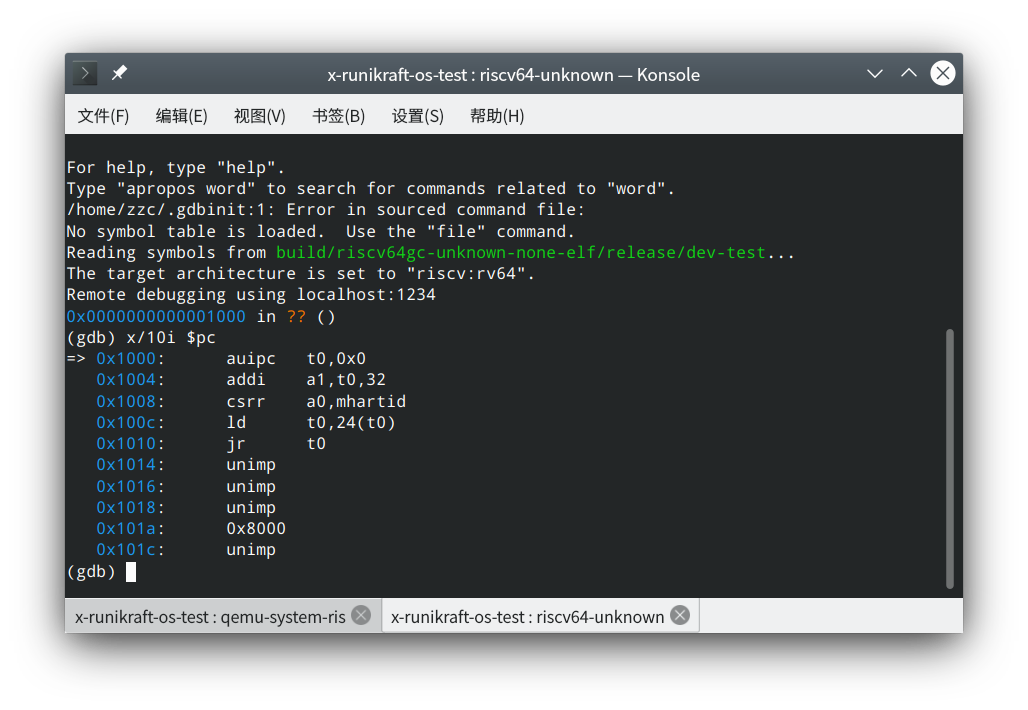
\includegraphics[width=0.9\linewidth]{assets/debug.png}
\vspace*{-3ex}
\caption{调试}
\label{fig:debug}
\end{figure}

\begin{figure}[tbh!]
\centering
\vspace*{-3ex}
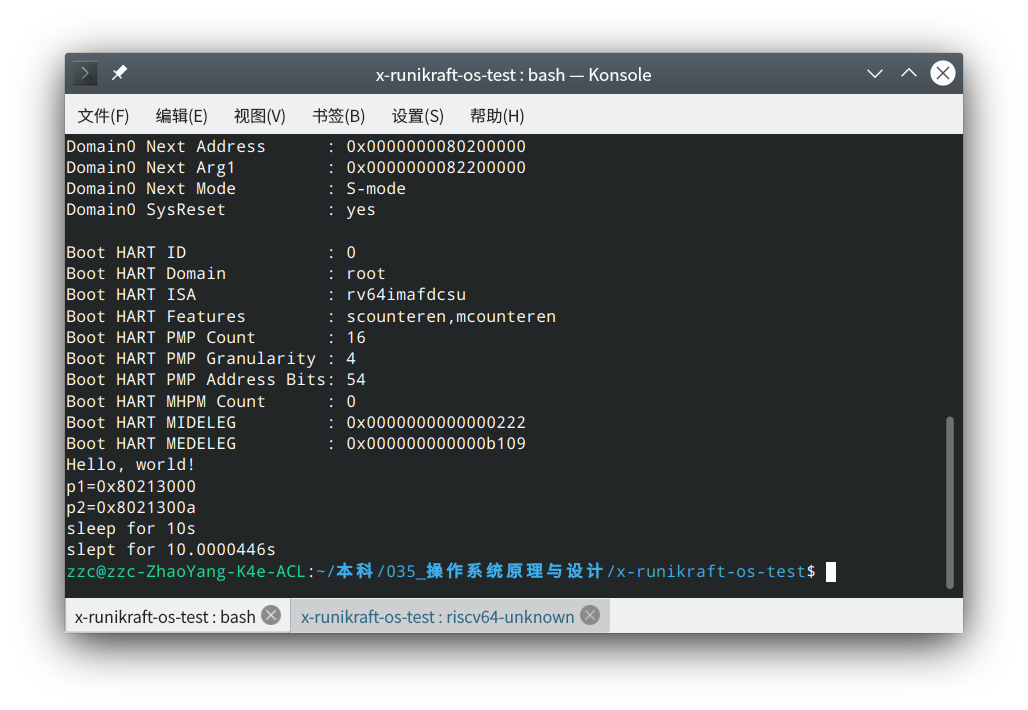
\includegraphics[width=0.9\linewidth]{assets/run.png}
\vspace*{-3ex}
\caption{运行结果}
\label{fig:run}
\end{figure}

\subsection{QEMU性能测试}
Unikernel以高性能著称,性能也是评价unikernel的重要指标。
然而遗憾的是,由于我们无法得到RISC-V物理机,而QEMU仿真硬件架构本身
会带来巨大的性能损失,所以我们很难准确评估我们写的Runikraft的性能。
为了相对准确的估计Runikraft
的性能,可以测试QEMU仿真本身带来的性能损失,
然后可以用QEMU上的运行时间除以性能损失比\footnote{riscv64时间÷ x86-64时间},估计真实RISC-V
硬件上的运行时间。

我们用组员张子辰同学的数据结构课程的大作业
\href{https://github.com/WCIofQMandRA/huffman_compressor}{Huffman树压缩器}做了基准测试。
测试结果见表\ \ref{table:test}。
\begin{longtable}{|c||>{\ttfamily}r|>{\ttfamily}r|>{\ttfamily}r||>{\ttfamily}r|>{\ttfamily}r|>{\ttfamily}r|}
\caption{QEMU基准测试}\label{table:test}\\
\hline
\multirow{2}{*}{文件}&\multicolumn{3}{c|}{压缩/s}&\multicolumn{3}{c|}{提取/s}\\\cline{2-7}
&\multicolumn{1}{c|}{x86-64}&\multicolumn{1}{c|}{riscv64}&\multicolumn{1}{c||}{损失比}&
\multicolumn{1}{c|}{x86-64}&\multicolumn{1}{c|}{riscv64}&\multicolumn{1}{c|}{损失比}\\\hline
\endfirsthead
test01&0.019& 0.079&4.16&0.009&0.058&6.44\\\hline
test02&0.040& 0.134&3.35&0.011&0.083&7.55\\\hline
test03&1.075& 3.054&2.84&0.316&1.624&5.14\\\hline
test04&1.114& 3.285&2.95&0.272&1.701&6.23\\\hline
test05&0.715& 2.085&2.92&0.201&1.116&5.55\\\hline
test06&5.001&14.121&2.82&1.177&7.018&5.96\\\hline
\end{longtable}

测试脚本是\href{https://github.com/WCIofQMandRA/huffman_compressor/blob/8ab200b656a0e087e27480fcbcae4000a59f6b47/test/benchmark.sh}{test/bencmark.sh}。
原始记录见我们的仓库的\href{https://github.com/OSH-2022/x-runikraft/tree/eca8a7575be96fb0a4dc311a8c60622c0e9b0aa5/reference/qemu-benchmark.log}{reference/qemu-benchmark.log}。

从测试结果可以看出,不同类型的程序的损失比并不相同,但是我目前并没有弄清楚
什么样的程序更容易造成性能损失。由于QEMU无法有效利用处理器的分支预测和高速缓存,
我猜测流水线友好和缓存友好的程序会引起较大的性能损失。考虑到内核的大部分操作不涉及大范围的
寻址,可以认为系统内核属于会引起较大性能损失的程序,所以我们把QEMU仿真带来的性能损失视为5。

\section{创新点}
与先前用Rust改写FreeRTOS的小组类似,我们的项目偏重工程,没有理论上的创新点。
由于我们了解的所有用Rust写的操作系统都或多或少的使用了unstable的特性,我们用stable特性
编写unikernel也不失为一种技术上的创新。

\section{概要设计}\sectionauthor{张子辰}\vspace*{-4ex}
\subsection{架构}
Runikraft的架构与Unikraft几乎相同。
\begin{figure}[!hbt]
\centering
\begin{minipage}{0.49\linewidth}
\centering
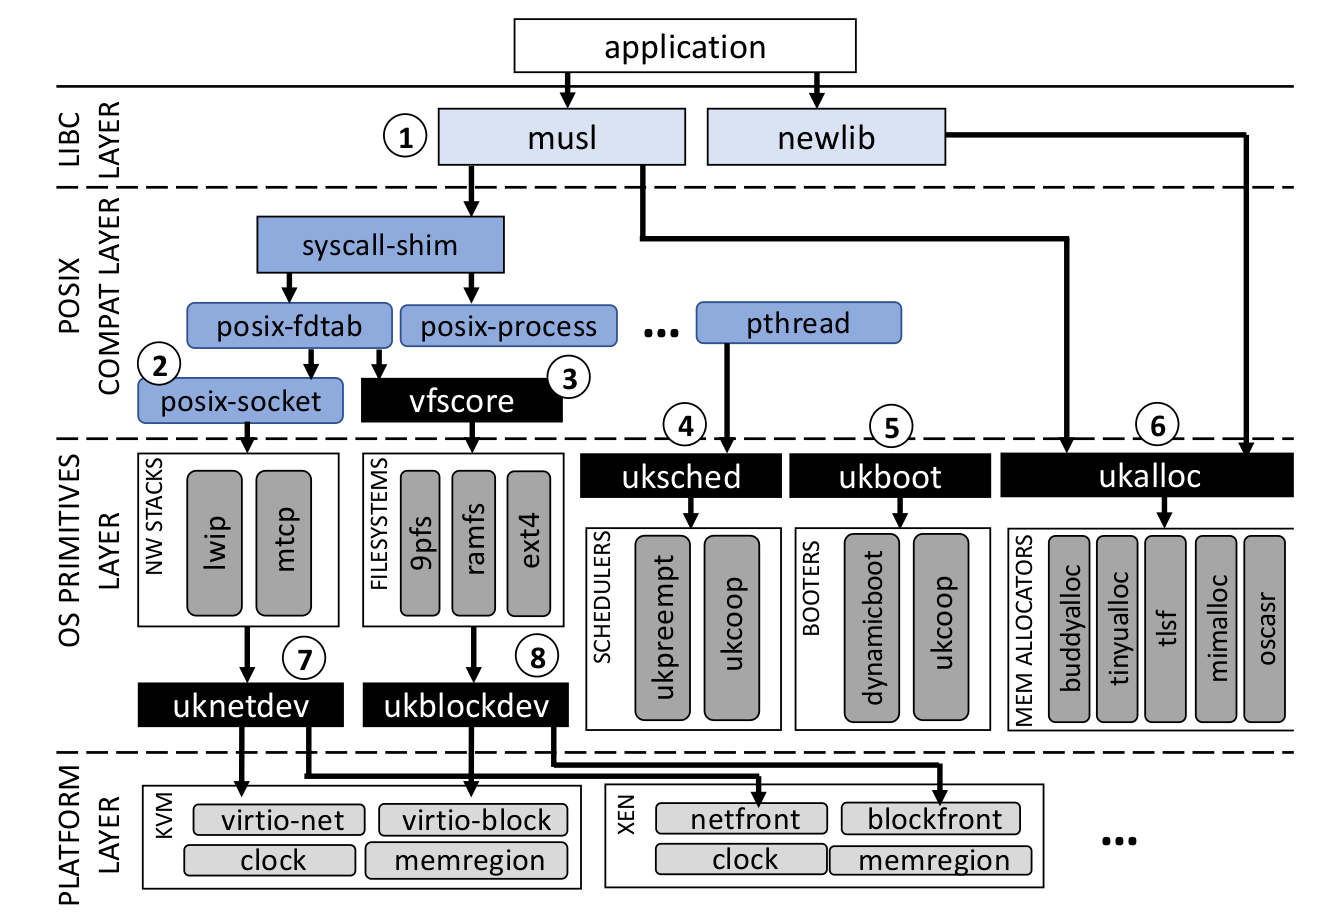
\includegraphics[width=\linewidth]{assets/Unikraft-architecture.png}
\caption{Unikraft的架构}\label{fig:unikraft-arch}
\end{minipage}
\begin{minipage}{0.49\linewidth}
\centering
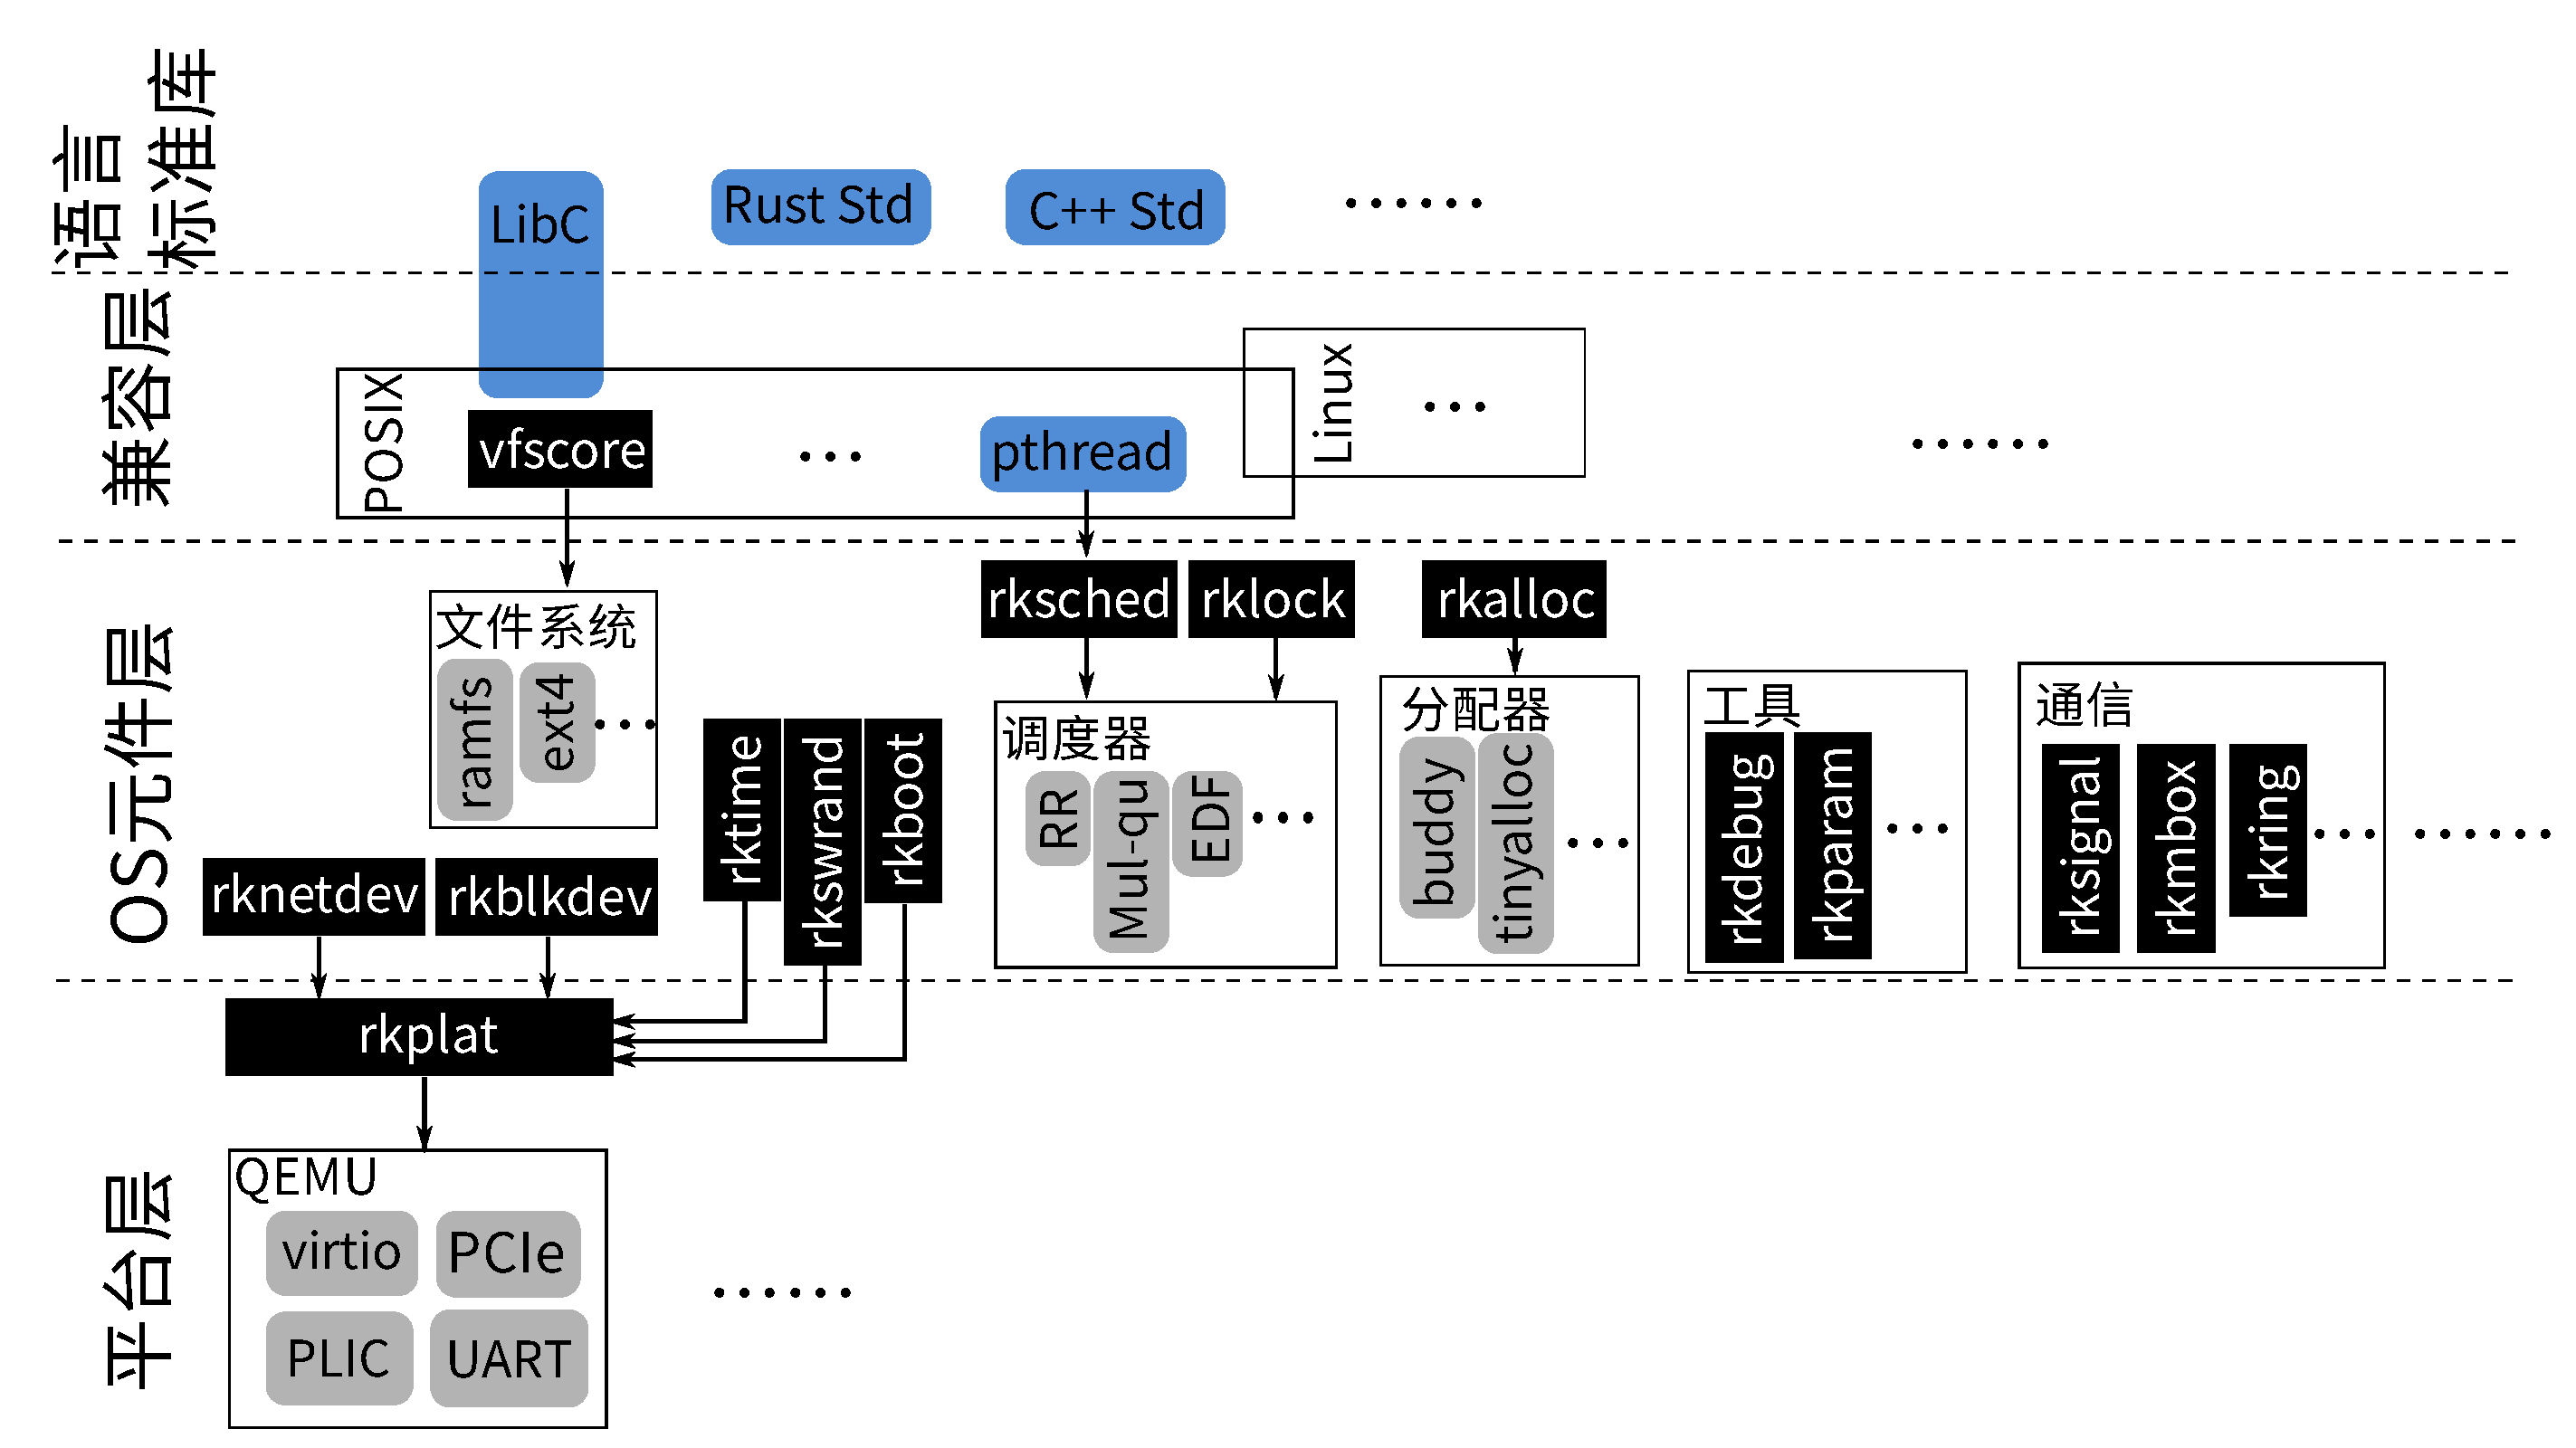
\includegraphics[width=\linewidth]{assets/Runikraft-architecture.pdf}
\caption{Runikraft的架构}\label{fig:runikraft-arch}
\end{minipage}
\end{figure}
平台层将不同的平台封装成通用的\texttt{rkplat} API,它提供与平台/架构密切相关的功能,
比如外设驱动、外中断处理、内存分页、定时器、原子操作、内存屏障,我们只计划支持RISC-V+QEMU virt
一种平台。如果时间不足,我们可以将现成的OpenSBI\cite{5}\cite{6}封装成\texttt{rkplat} API。

\texttt{rknetdev}、\texttt{rkblkdev}、\texttt{rktime}、\texttt{rkswrand}、\texttt{rkboot}
五个APIs的功能与平台密切相关,
但是为了降低开发和维护难度,它们并没有直接实现,而是在\texttt{rkplat}提供的初级抽象的基础上实现。
\texttt{rknetdev}和\texttt{rbblkdev}对应图\ \ref{fig:unikraft-arch}\ 的⑦和⑧,
它们分别提供网络设备和块设备的支持。
%与Unikraft的实现类似,这两个APIs的构造函数的参数接受指向\texttt{trait RKplat}的指针。
\texttt{rktime}提供获取和修改系统时间的API,\texttt{rkswrand}提供密码学安全的随机数,
\texttt{rkboot}负责完成OS元件的初始化并将控制权转交给用户的代码。

\texttt{rksched}和\texttt{rklock}是两个与调度器有关的APIs,前者负责创建、调度、撤销线程,后者负责线程间
的同步和互斥。Runikraft支持多种调取器,比如,图\ \ref{fig:runikraft-arch}\ 中的RR是时间片轮转调度器、
Mul-qu是多重队列调取器、EDF是截止日期有限调度器。我们计划先实现RR调度器。当然,为了系统镜像的轻量性,
用户可以不使用任何调取器,这时,\texttt{rksched}和\texttt{rklock}会被编译成空API,创建线程的行为
将和函数调用相同。这保证了大部分使用仅仅并行加速的程序仍然能正确运行。

Runikraft选择性地提供线程通信模块,如UNIX风格的信号(\texttt{rksignal}),信箱(\texttt{rkmbox}),
无锁的环形缓冲队列(\texttt{rkring})。

我们目前没有计划区分线程和进程,Runikraft的线程同时具有传统的OSes的线程和进程的特性:
线程之间没有隔离措施,但是线程之间又可以使用进程通信的方法更安全地同步。

\texttt{rkalloc}是分配器API,它的后端可以是\texttt{buddy}、\texttt{tinyalloc}、\texttt{tlsf}、
\texttt{mimalloc}等分配器。
不过,我们可能只会实现其中的一个。

Runikraft还提供了一些工具模块,比如调试工具\texttt{rkdebug}、命令行参数分析工具\texttt{rkparam}。

在 Unikraft 中,文件系统 API vfscore 是 POSIX 兼容层的一部分,我们沿用了它的设
计,将 \texttt{vfscore} 放在了兼容层。Runikraft计划支持RAM上的临时文件系统和Plan 9 OS的9fps。

位于最顶层的是语言标准库,这一层可以帮助Runikraft支持多种语言。
虽然语言标准库层被画在了兼容层之上,但它其实是直接用OS元件层的APIs实现的,这能避免分层系统
的低效。
我们只打算实现Rust标准库和C标准库的部分内容。

\subsection{改写方法}

\subsubsection{类型转换}
下面是通常情况下Unikraft使用的C类型对应的Rust类型。
越先出现的规则优先级越高,即如果一个C类型与多条规则匹配,则按最先出现的规则转换
成Rust类型,但是如果转换后的类型会引起所有权问题,则放弃这条转换规则,按下一条匹配的
规则转换。
\begin{longtable}{|l|l|}
\caption{}\\
\hline
C类型&Rust类型\\\hline
\endfirsthead
\hline
C类型&Rust类型\\\hline
\endhead
\texttt{long}&\texttt{isize}\\\hline
\texttt{unsigned long}&\texttt{usize}\\\hline
\texttt{\_\_sz}&\texttt{usize}\\\hline
\texttt{\_\_nsec}&\texttt{core::time::Duration}\\\hline
代表错误信息的\texttt{int}&\texttt{Result<(),i32>}\\\hline
取1或0的\texttt{int}&\texttt{bool}\\\hline
\texttt{T[N]}&\texttt{[T;N]}\\\hline
\texttt{void \_\_noreturn}&\texttt{!}\\\hline
\texttt{void*}&(泛型函数)\texttt{*mut T}\\\hline
\texttt{void*}&(泛型函数)\texttt{*const T}\\\hline
\texttt{void*}&\texttt{*const u8}\\\hline
\texttt{void*}&\texttt{*mut u8}\\\hline
\texttt{const char*}&\texttt{\&str}\\\hline
传递结果的\texttt{T*},返回\texttt{int}&\texttt{Result<T,int>}或\texttt{Optional<T>}\\\hline
传递结果的\texttt{T*},返回\texttt{void}&\texttt{T}\\\hline
\texttt{T*}+\hspace{0cm}长度&\texttt{\&mut [T]}\\\hline
\texttt{const T*}+\hspace{0cm}长度&\texttt{\&[T]}\\\hline
\texttt{T*}&\texttt{\&mut T}\\\hline
\texttt{T*}&\texttt{*mut T}\\\hline
\texttt{const T*}&\texttt{\&T}\\\hline
\texttt{const T*}&\texttt{*const T}\\\hline
整型&长度和符号相同的整型\\\hline
浮点类型&长度相同的浮点类型\\\hline
\end{longtable}

Unikraft用到了少量双重指针。一般地,C的双重指针\texttt{T**}在C++的含义是\texttt{T \&*},
所以它对应Rust的\texttt{\&mut *mut T}。但是这种写法比较丑陋,所以我们会尽量通过改写
函数传参的方式,避免使用指针的引用。

\subsubsection{面向对象式函数}
所谓“面向对象式函数”就是\ \ref{ssubsec:code-style}\ 提到的第一个参数是
与库同名的结构体的指针的函数。在Rust中,可以把这些函数放在\texttt{\textbf{impl}}块
中,第一个参数是\texttt{\textbf{self}}。

如\texttt{ukring}的入队操作
\begin{lstlisting}[language=C]
static __inline int
uk_ring_enqueue(struct uk_ring *br, void *buf)
{
    /* 实现略 */
}
\end{lstlisting}
改写为
\begin{lstlisting}[language=Rust]
impl Ring {
    fn enqueue<T>(&mut self, buf: *const T)->Result<(),i32> {
        // 实现略
    }
}
\end{lstlisting}

\subsubsection{宏}

用\ \ref{subsec:cond-compile}\ 的方法处理条件编译宏。
把宏常量转换为静态变量。把仿函数宏转换成内联函数,在必要时使用泛型。
把用宏实现的模板类型转换成基于泛型的结构体,它们主要是链表这样的容器。

\subsubsection{编译提示}
Rust的中的\texttt{cold}属性可以充当GCC中的\texttt{\_\_builtin\_expect(\textit{<expr>},0)},
也就是\texttt{unlikely(\textit{<expr>})},但是Rust中没有含义是\texttt{likely}的属性。

GCC的\texttt{\_\_inline}等价于Rust的\texttt{\#[inline]},
GCC的\texttt{\_\_attribute\_\_((always\_inline))}等价于Rust的\texttt{\#[inline(always)]},
GCC的\texttt{\_\_attribute\_\_((no\_inline))}等价于Rust的\texttt{\#[inline(never)]}。

一些依赖布局的结构体,如\texttt{\_\_regs}改写成Rust后需要附加\texttt{\#[repr(C)]}属性,
以确保能直接通过偏移量访问结构体成员。
\subsection{时间安排}
以星期日为一周的起点。大体上,第10\tildechar14周实现OS元件层,第15、16周实现兼容层,具体安排见
表\ \ref{table:schedule}。
\begin{table}[!hbt]
\centering
\caption{时间安排}\ \label{table:schedule}
\begin{tabular}{|r|l|l|l|l|l|}
\hline
第10周&\multirow{2}{*}{\texttt{rkplat}}&\texttt{rkalloc}&\multirow{2}{*}{\texttt{rkring}}&\multirow{3}{*}{\texttt{rkblkdev}}&\texttt{rksched}\\\cline{1-1}\cline{3-3}
第11周&&\multirow{3}{*}{\texttt{rknetdev}}&&&无抢占\\\cline{1-2}\cline{4-4}\cline{6-6}
第12周&\texttt{rktime}&&\multirow{2}{*}{\texttt{rkmbox}}&&\texttt{rklock}\\\cline{1-2}\cline{5-6}
第13周&\texttt{rkswrand}&&&\multirow{2}{*}{9pfs}&\texttt{rksched}\\\cline{1-4}
第14周&\texttt{rkplat}&\texttt{rkparam}&\texttt{rksignal}&&可抢占\\\cline{1-1}\cline{3-6}
第15周&不依赖&\multirow{2}{*}{RustStd}&\multirow{2}{*}{LibC}&\multirow{2}{*}{\texttt{vfscore}}&\multirow{2}{*}{\texttt{pthread}}\\\cline{1-1}
第16周&SBI&&&&\\\hline
\end{tabular}
\end{table}

\section*{许可协议}
本文档以知识共享署名 4.0 国际 (CC BY 4.0)许可证发布。

\vspace{2ex}
\noindent\textbf{\large 您可以自由地}:
\begin{description}
\item[共享] 在任何媒介以任何形式复制、发行本作品;
\item[演绎] 修改、转换或以本作品为基础进行创作
在任何用途下,甚至商业目的。
\end{description}

\vspace{2ex}
\noindent\textbf{\large 惟须遵守下列条件}:
\begin{description}
\item[署名] 您必须给出适当的署名,提供指向本许可协议的链接,
同时标明是否(对原始作品)作了修改。您可以用任何合理的方式来署名,
但是不得以任何方式暗示许可人为您或您的使用背书。
\item[没有附加限制] 您不得使用法律术语或者技术措施,从而限制其他人
做许可协议允许的事情。
\end{description}

\vspace{2ex}
\noindent\textbf{\large 声明}:

您不必因为公共领域的作品要素而遵守许可协议,或者您的使用被可适用的例外或限制所允许。

不提供担保。许可协议可能不会给与您意图使用的所必须的所有许可。
例如,其他权利比如形象权、隐私权或人格权可能限制您如何使用作品。

本许可证的全文位于:\\
\centerline{\url{https://creativecommons.org/licenses/by/4.0/legalcode.zh-Hans}}
\bibliographystyle{IEEEtran}
\bibliography{feasibility-report.bib}
\end{document}
